\documentclass{ctexart}

% 导言区

%% 必备宏包
\usepackage{amsmath}
\usepackage{amssymb} % 数学符号
\usepackage{graphicx}
\usepackage{float} % 取消浮动机制
\usepackage{anyfontsize}

%% 可选宏包
\usepackage{hyperref}
\usepackage{gbt7714}
\usepackage{color}
\usepackage{amsthm} % 定理环境

%% 初始化设置
\bibliographystyle{gbt7714-numerical}
\numberwithin{equation}{section}
\numberwithin{figure}{section}
\newtheorem{myEx}{Example}[section] % 定义一个 myEx 的定理环境
\newtheorem{myDef}{Definition}[section]
\newtheorem{myThm}{Theorem}[section]

%% 初始化标题页
\title{MIT18.01:\ Single Variable Calculus}
% 添加一个副标题{Lecture Notes}
\author{Borne}
\date{\zhtoday}

% 正文
\begin{document}

%% 标题
\maketitle
\thispagestyle{empty}

%% 目录
\newpage
\tableofcontents
\thispagestyle{empty}
\newpage
\setcounter{page}{1}

%% 正文内容
\newpage
\section{Unit One:\ Derivative}
\subsection{什么是导数}
\subsubsection{导数的几何解释}
对于一个函数曲线 \(f(x)\),如何求曲线上一点\(P\)的切线「tangent line」?

\begin{figure}[H]
    \centering
    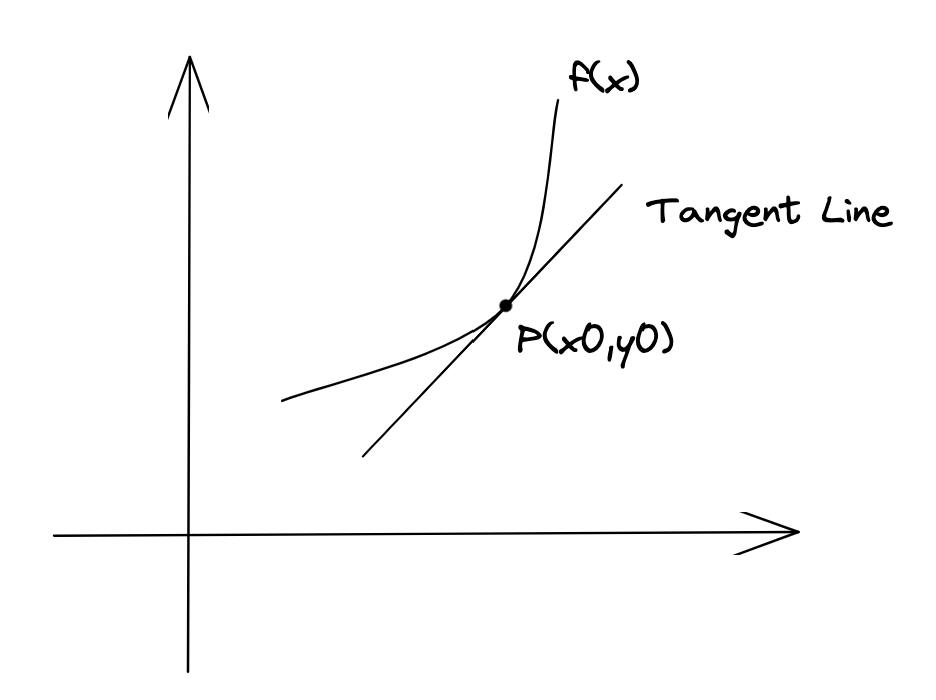
\includegraphics[scale=0.45]{images/tagentline.png}
    \caption{函数的切线}
\end{figure}

对于上图所展示的情况,通过「点斜式」给出切线的方程是最好的选择,即:在已知直线上一点\(P(x_0,y_0)\)
\begin{equation}
    y - y_0 = k(x - x_0)
\end{equation}
为了给出切线方程,还需要找到切线的斜率 \(k\),该如何求?

这时候不妨再在曲线 \(f(x)\) 引入一点 \(Q\),可以得到曲线 \(f(x)\) 的一条割线「secant line」
\begin{figure}[H]
    \centering
    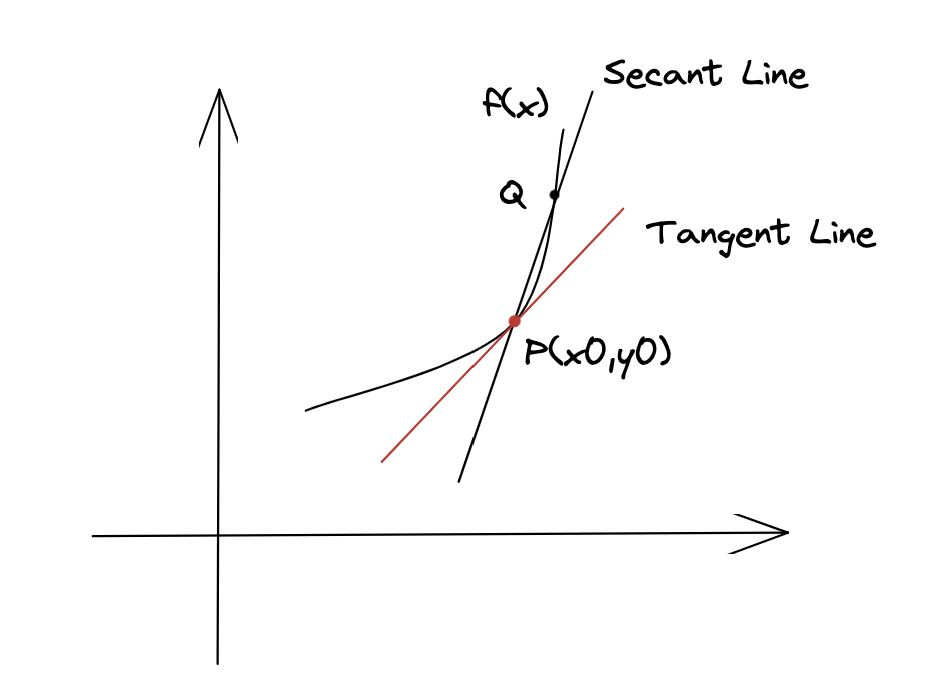
\includegraphics[scale=0.45]{images/introduceSecantLine.png}
    \caption{函数的割线}
\end{figure}

很容易发现,当 \(Q\) 点逐渐向 \(P\) 点移动时,上图中「割线」会逐渐逼近「切线」,而对于「割线」的方程是很容易给出的。

下面,试着用数学语言来描述这一变化的过程:
\begin{equation}
    k = \lim\limits_{\Delta x \to 0} \frac{\Delta f}{\Delta x}\label{eq:Deltaf/DeltaX}
\end{equation}
利用「割线」的斜率「slope」去逼近「切线」的斜率。
\begin{figure}[H]
    \centering
    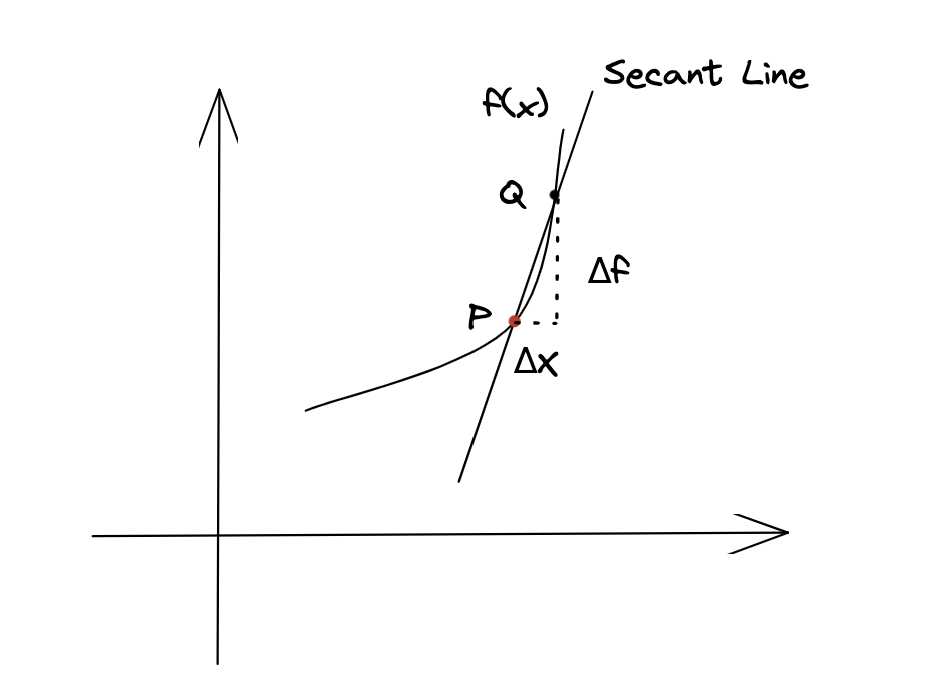
\includegraphics[scale=0.45]{images/ScantL_Llimit_TangentL.png}
    \caption{用割线逼近切线}
\end{figure}

根据 (\ref{eq:Deltaf/DeltaX}) 式,可以得到,曲线 \(f(x)\) 上任意一点 \(x_0\)处导数
\footnote{注意,关于导数的记号主要存在以下两种:
    \begin{itemize}
        \item Newton的记号:
              \( f^{\prime} \)
        \item Leibniz的记号:
              \( \frac{df}{dx}=\frac{dy}{dx}=\frac{d}{dx}f=\frac{d}{dx}y \)
    \end{itemize}}的定义:
\begin{equation}
    f^{\prime}(x_0) = \lim\limits_{\Delta x \to 0}\frac{f(x_0 + \Delta x) - f(x_0)}{\Delta x}
\end{equation}

\begin{myDef}\label{Def:Derivative}
    \(f(x)\): Derivative at \(x_0\)
    \begin{equation*}
        f^{\prime}(x_0) = \lim\limits_{\Delta x \to 0}\frac{f(x_0 + \Delta x) - f(x_0)}{\Delta x}
    \end{equation*}
    Another equivalent definition:
    Let \(\Delta x = x - x_0\)
    \begin{equation*}
        f^{\prime}(x_0) = \lim\limits_{ x - x_0 \to 0}\frac{f(x_0 +  x - x_0) - f(x_0)}{ x - x_0} = \lim\limits_{ x \to x_0}\frac{f(x) - f(x_0)}{ x - x_0}
    \end{equation*}
    Maybe:Let \(\Delta y = f(x_0 + \Delta x) - f(x_0)\)
    \begin{equation*}
        f^{\prime}(x_0) = \lim\limits_{\Delta x \to 0}\frac{\Delta y}{\Delta x}
    \end{equation*}
\end{myDef}

\begin{myEx}\label{Ex:1/x}
    \quad \( f(x) = \frac{1}{x}\)
    \begin{equation*}
        f^{\prime}(x_0) = \lim \limits_{\Delta x \to 0}\frac{f(x_0 + \Delta x) - f(x_0)}{\Delta x} = \frac{\frac{1}{x_0 + \Delta x} - \frac{1}{x_0}}{\Delta x} = -\frac{1}{x_0^{2}}
    \end{equation*}
\end{myEx}

\begin{myEx}\label{Ex:x^{n}}
    \quad \( f(x) = x^{n} \),其中,\(n = 1,2,3, \cdots\),即:\(n \in N^{*}\)
    \begin{equation*}
        f^{\prime}(x) = \lim_{\Delta x \to 0}\frac{(x + \Delta x)^{n} - x^{n}}{\Delta x}
    \end{equation*}
    其中,\( (x + \Delta x)^{n} \) 通过二项式定理展开
    \begin{equation*}
        (x + \Delta x)^{n} = \binom{n}{0}x^{n} (\Delta x)^{0} + \binom{n}{1}x^{n-1} (\Delta x)^{1} +  \mathcal{O}((\Delta x)^{2})
    \end{equation*}
    将展开的结果带入到求导的式子中去,有:
    \begin{equation*}
        f^{\prime}(x) = \lim_{\Delta x \to 0}\frac{x^{n} + nx^{n-1}\Delta x + \mathcal{O}((\Delta x)^{2}) - x^{n}}{\Delta x} = nx^{n-1}
    \end{equation*}
\end{myEx}
结合 Example \ref{Ex:1/x} 和 Example \ref{Ex:x^{n}} 的结果,可以得到:
\begin{equation}\label{eq:x^{n}}
    \frac{d}{dx}x^{n} = nx^{n-1}, \text{其中,} n \in Z
\end{equation}

\subsubsection{导数的物理解释}\label{sec:Derivative's physics interpretation}

导数的实质是要看某个量的微小变化,以及它和它所导致的另一个量的微小变化有什么关系\cite[1:11]{3Blue1Brown03YongJiHeLaiQiuDao2018},也即是通常所说的变化率「rate of change」。

在物理上,当用到导数时,一般都是想从物质的平均变化「average change」中去窥探物质的瞬时变化「instantaneous change」,比如:
\begin{itemize}
    \item \(q = charge,\quad \frac{dq}{dt} = current\)
    \item \(s=distance,\quad \frac{ds}{dt} = speed\)
    \item \(T =temperature,\quad \frac{dT}{dx} = temperature \ gradient\)
    \item \(sensitive \  of \  measurement\)
\end{itemize}

\subsection{导数、极限和连续}

\subsubsection{极限「Limitation」}
在 (\ref{eq:Deltaf/DeltaX}) 式中,为了定义导数引入了极限「limitation」的概念。极限一般可以分为以下两种类型:
\begin{itemize}
    \item 简单极限\footnote{注意:当\(\lim\limits_{x \to 4}\),就已经代表永远不考虑 \(x=4\) 的情况,即使 \(x=4\) 处没有定义,也不会造成任何影响,\(x\) 取的只是一个非常逼近 \(4\) 的值,比如:\(x=4.00000001\).}
          \begin{equation*}
              \lim_{x \to 4} \frac{x + 2}{x^2 + 3} = \frac{6}{19}
          \end{equation*}
    \item 导数类型的极限(即:“\(\frac{0}{0}\)” \  型极限)
          \begin{equation*}
              \lim_{\Delta x \to 0} \frac{f(x + \Delta x) - f(x)}{\Delta x}
          \end{equation*}
\end{itemize}
不难发现,对于「简单极限」可以直接进行求解;但对于「导数类型的极限」,在求解之前需要先对式子进行一些处理。

还有一种极限的分类方式,根据逼近的方向,可以将极限分为:
\begin{itemize}
    \item 左极限:表示过去
          \begin{equation*}
              \lim\limits_{x \to x_0^{-}}f(x)
          \end{equation*}
    \item 右极限:关乎未来
          \begin{equation*}
              \lim\limits_{x \to x_0^{+}}f(x)
          \end{equation*}
\end{itemize}
这里需要注意的是,通常提到的函数在某一点极限存在,比如:
\begin{equation*}
    \lim\limits_{x \to x_0}f(x) = a
\end{equation*}
具体是指:
\begin{equation*}
    \lim\limits_{x \to x_0^{-}}f(x) = \lim\limits_{x \to x_0^{+}}f(x) = a
\end{equation*}
也即是:
\begin{equation*}
    \lim\limits_{x \to x_0}f(x) = a \Leftrightarrow
    \lim\limits_{x \to x_0^{-}}f(x) = \lim\limits_{x \to x_0^{+}}f(x) = a
\end{equation*}
说明通过一个点的左、右极限,可以判断该点的极限是否存在!

\subsubsection{连续「Continuity」}
为了定义导数,引入了极限,有了极限的概念之后,还可以进一步定义函数的连续「Continuity」.
\begin{myDef}\label{Def:Continuity}
    Continuity at \(x_0\):
    \begin{equation*}
        \lim\limits_{x\to x_0}f(x) = f(x_0)
    \end{equation*}
\end{myDef}
上面关于在某点处连续的定义,其实包含了 \(3\) 层意思:
\begin{itemize}
    \item \(\lim\limits_{x\to x_0}f(x)\) 存在,也即是:\(\lim\limits_{x \to x_0^{-}}f(x) = \lim\limits_{x \to x_0^{+}}f(x)\);
    \item \(f(x)\) 在 \(x = x_0\)处有定义;
    \item 两者相等,即:\(f(x)\) 在 \(x = x_0\)处的极限正好等于\(f(x)\)在\(x = x_0\)处的函数值。
\end{itemize}
根据函数在某一点连续时的 \(3\) 层含义,可以进一步分析出函数在某一点处不连续时的情况:
\begin{itemize}
    \item 跳跃间断点「jump discontinuity」

          左、右极限均存在,但不相等。
    \item 可去间断点「removable discontinuity」

          \(\lim\limits_{x \to x_0^{-}}f(x) = \lim\limits_{x \to x_0^{+}}f(x)\),但 \(f(x)\) 在 \(x = x_0\)处无定义,比如:
          \begin{equation*}
              g(x) = \frac{\sin x}{x} \quad \text{或} \quad h(x)=\frac{1-\cos x}{x}
          \end{equation*}

    \item 无穷间断点「infinite discontinuity」
          \[ f(x) = \frac{1}{x},\quad \lim\limits_{x\to 0^{-}}\frac{1}{x} = -\infty, \quad \lim\limits_{x\to 0^{+}}\frac{1}{x} = +\infty\]
    \item 另类丑陋间断点「other ugly discontinuity」
          \[ y = \sin \frac{1}{x} \quad \text{当}   x \to 0 \text{时,不存在左、右极限。}  \]

\end{itemize}

\subsubsection{导数与极限、连续的关系}
导数不管是对于极限,还是连续来说,都具有重要意义。对于极限来说,在后面会看到,\textcolor{red}{通过导数(洛必达法则)可以去求极限};对于连续来说,有下面的定理:
\begin{myThm}[Diff \(\Rightarrow\) CTS]\label{Thm:DiffCTS}
    可导必连续
\end{myThm}
\begin{proof}
    已知函数 \(f(x)\) 可导,需要证明 \(f(x)\) 连续。

    根据 Definition \ref{Def:Continuity} 中连续的定义,可以得到 \(f(x)\) 连续的等价证明:
    \begin{equation*}
        \lim\limits_{x\to x_0}f(x) - f(x_0) = 0
    \end{equation*}

    从 \(\lim\limits_{x\to x_0}f(x) - f(x_0)\) 出发,对其进行等价变换,有:
    \begin{equation*}
        \lim\limits_{x\to x_0}f(x) - f(x_0) = \lim\limits_{x\to x_0}\frac{f(x) - f(x_0)}{x - x_0}(x - x_0)
    \end{equation*}
    已知条件 \(f(x)\) 可导,根据 Definition \ref{Def:Derivative} 中给出的导数的定义,有:
    \begin{equation*}
        \lim\limits_{x\to x_0}f(x) - f(x_0) = \lim\limits_{x\to x_0}\frac{f(x) - f(x_0)}{x - x_0}(x - x_0) =
        f^{\prime}(x_0)\lim\limits_{x\to x_0}(x - x_0) = 0
    \end{equation*}
    \textcolor{red}{注意}:这个部分用到了\textcolor{red}{极限的四则运算},有待补充!
\end{proof}

\begin{myEx}\label{Ex:CTSNotDiff}
    连续但不可导
    \begin{equation*}
        f(x) = \left| x \right| =
        \begin{cases}
            x,  & x \geq 0 \\
            -x, & x < 0
        \end{cases}
    \end{equation*}
    显然,在 \(x = 0\) 点处, \(f(x)\) 连续:
    \begin{equation*}
        \lim\limits_{x\to 0} f(x)  = \lim\limits_{x\to 0} \left| x \right| = f(0) = 0
    \end{equation*}
    但是,在 \(x = 0\) 点处,\(f(x)\) 并不可导,根据 Definition \ref{Def:Derivative} 导数的定义,有:
    \begin{equation*}
        \lim\limits_{x\to 0}\frac{f(x) - f(0)}{x - 0} = \lim\limits_{x\to 0}\frac{\left| x \right|}{x} =
        \begin{cases}
            1,  & x \to 0^{+} \\
            -1, & x \to 0^{-}
        \end{cases}
    \end{equation*}
    说明 \(\lim\limits_{x\to 0^{-}} \neq \lim\limits_{x\to 0^{+}}\) , \(\lim\limits_{x\to 0}\frac{f(x) - f(0)}{x - 0}\)不存在,即:\(f(x)\) 在 \(x = 0\) 点处不可导。
    \begin{figure}[H]
        \centering
        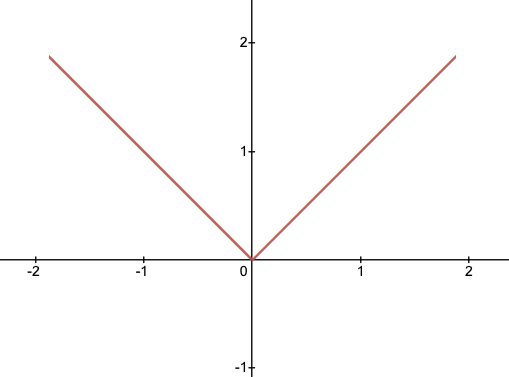
\includegraphics[scale=0.4]{images/abs(x).png}
    \end{figure}
\end{myEx}
Theorem \ref{Thm:DiffCTS} 和 Example \ref{Ex:CTSNotDiff} 共同说明了,「可导」是比连续更强(或更好)的条件,它使得函数不但连续,而且更光滑!

\subsection{求导的一般法则}

\subsubsection{加法法则}
\begin{equation}
    (u + v)^{\prime} = u^{\prime} + v^{\prime}
\end{equation}

\subsubsection{乘法法则}
\begin{equation}
    (uv)^{\prime} = u^{\prime}v + uv^{\prime}
\end{equation}

\subsubsection{链式法则}
设 \( w = f(v)\),\(v = u(x) \),有:
\begin{equation}
    \frac{dw}{dx} = \frac{dw}{dv} \frac{dv}{dx} = f^{\prime}(v)v^{\prime}
\end{equation}

下面,直观说明一下链式法则「Chain Rule」的正确性:
\begin{align*}
    \begin{cases}
        y = 10x + b, & \frac{dy}{dx} = 10 \\
        x = 5t + a,  & \frac{dx}{dt} = 5
    \end{cases}
    \Rightarrow
    \begin{cases}
        y = 10(5t + a) + b = 50t + 10a + b \\
        \frac{dy}{dt} = 50 = \frac{dy}{dx}\cdot \frac{dx}{dt}
    \end{cases}
\end{align*}

\subsubsection{隐函数微分}\label{sec:Implicit Differentiation}

对于所有显函数\footnote{以直接用含自变量的算式表示的函数称为显函数},形如:\(y=f(x)\),均可以进行求导;但是对于隐函数,形如:\(F(x,y) = 0\),求导是非常困难的。通常对隐函数求导,我们的选择是利用隐函数微分「Implicit Differentiation」的方法进行求导。

\begin{myEx}\label{Ex:x^{m/n}}
    \(y = x^{\frac{m}{n}}\),其中,\(m,n\in Z\)

    借助于已知函数的导数(\ref{eq:x^{n}} 式),将 \(y = x^{\frac{m}{n}}\) 转换为隐函数的形式,利用隐函数微分进行求导:
    \begin{align*}
        y = x^{\frac{m}{n}}   & \Rightarrow y^{n} = x^{m}   \\
        \frac{d}{dx}y^{n}     & = \frac{d}{dx}x^{m}         \\
        ny^{n-1}\frac{d}{dx}y & = mx^{m-1}                  \\
        \frac{d}{dx}y         & = \frac{mx^{m-1}}{ny^{n-1}}
    \end{align*}
    最后,再将原式 \(y = x^{\frac{m}{n}}\) 代入,得到最后的结果:
    \begin{equation}
        \frac{d}{dx}x^{\frac{m}{n}} = \frac{mx^{m-1}}{ny^{n-1}} = \frac{mx^{m-1}}{nx^{\frac{m(n-1)}{n}}} = \frac{m}{n}x^{\frac{m}{n} - 1}
    \end{equation}
\end{myEx}
至此,结合 Example \ref{Ex:1/x}, Example \ref{Ex:x^{n}} 和 Example \ref{Ex:x^{m/n}} 的结果,可得:
\begin{equation}
    \frac{d}{dx}x^{n} = nx^{n-1}, \text{其中,} n \in Q
\end{equation}

\begin{myEx}
    \(x^{2} + y^{2} = 1\)
    \begin{align*}
        \frac{d}{dx}\left(x^{2} + y^{2} = 1\right) \\
        2x + 2y\frac{d}{dx}y = 0                   \\
        \frac{d}{dx}y = - \frac{x}{y}
    \end{align*}
    可以发现,上面的形式并不是最终结果,还需要从 \(x^{2} + y^{2} = 1\) 中,将 \(y\) 解出来,代入上式:
    \begin{equation*}
        y = \pm \sqrt{1-x^{2}}
    \end{equation*}
    那么,就有:
    \begin{equation*}
        \frac{d}{dx}y = \mp \frac{x}{\sqrt{1-x^{2}}}
    \end{equation*}
\end{myEx}
从这个例子中可以发现,当一个隐函数无法显示化时,即使通过隐函数微分也无法得到最终的导数。即:得不到一个无法显示化的隐函数的导数。

当然,当一个隐函数可以显示化时,除了通过隐函数微分进行求导之外,还可以先将隐函数显示化,再对显示化的结果进行求导,但是,通常这样求导起来会比隐函数微分复杂。

\subsection{特殊函数的导数}

在开始求某一些由特定表达式表示出的函数的导数之前,先来谈一谈为什么学微积分,在大部分时间内都要纠缠于抽象函数的导数,而不是在考虑实实在在的变化率问题\cite{3Blue1Brown03YongJiHeLaiQiuDao2018}?

这是因为许多现实世界中的现象,许多我们想用微积分来分析的实际问题,都需要用到多项式,三角函数,指数函数,或其他的纯函数来描述。因此假如你能够熟练掌握这些抽象函数的变化率的思想,那你就学到了这门可以熟练精确地描述事物变化率的语言,并能够在任何你需要用微积分来模拟的实际问题中使用它。

\subsubsection{三角函数}\label{sec:trigfunc}

正弦函数 \(\sin x\) 的导数\footnote{由于\(\cos x\)的导数求法与\(\sin x\)的导数求法类似,所以就以\(\sin x\)的导数求法为例进行说明。},根据导数的定义 Definition \ref{Def:Derivative},有:
\begin{equation}\label{eq:DerivativeofSine}
    \begin{aligned}
        \frac{d}{dx}\sin x = & \lim\limits_{\Delta x \to 0}\frac{\sin(x + \Delta x) - \sin x}{\Delta x}                                                                    \\
        =                    & \lim\limits_{\Delta x \to 0}\frac{\sin x \cos\Delta x + \cos x \sin\Delta x  - \sin x}{\Delta x}                                            \\
        =                    & \lim\limits_{\Delta x \to 0} \left(\sin x\frac{\cos \Delta x - 1}{\Delta x}  + \cos x \frac{\sin \Delta x}{\Delta x} \right)                \\
        =                    & \sin x \lim\limits_{\Delta x \to 0} \frac{\cos \Delta x - 1}{\Delta x} + \cos x \lim\limits_{\Delta x \to 0} \frac{\sin \Delta x}{\Delta x}
    \end{aligned}
\end{equation}
不难发现,求 \(\sin x\) 的导数值,最终转换成了求下面两部分的极限值:
\begin{equation*}
    \lim\limits_{\Delta x \to 0} \frac{\sin \Delta x}{\Delta x} \quad \text{和} \quad \lim\limits_{\Delta x \to 0} \frac{\cos \Delta x - 1}{\Delta x}
\end{equation*}
再进一步转换,可以发现:
\begin{align}
     & \lim\limits_{\Delta x \to 0} \frac{\sin \Delta x}{\Delta x} =
    \lim\limits_{x \to 0} \frac{\sin x}{x} = \lim\limits_{x \to 0} \frac{\sin x  - \sin 0}{x - 0} = \left.\frac{d}{dx}\sin x\right|_{x=0}                                                                          \\
     & \lim\limits_{\Delta x \to 0} \frac{\cos \Delta x - 1}{\Delta x} = \lim\limits_{x \to 0} \frac{\cos x - 1}{x} = \lim\limits_{x \to 0} \frac{\cos x - \cos 0}{x - 0} = \left.\frac{d}{dx}\cos x \right|_{x=0}
\end{align}
即:通过求 \(\sin x\) 和 \(\cos x\) 在 \(x = 0\) 处的导数值,就可以推出\(\sin x\) 和 \(\cos x\)在其它所有点处的导数值。

下面,就来求一下 \(\sin x\) 和 \(\cos x\) 在 \(x = 0\) 处的导数值。用到了几何直观的方法。首先,求 \(\sin x\)
在 \(x = 0\) 处的导数值。从图 \ref{fig:sinx/x} 中可以得到以下结论\footnote{这里用到了弧长公式:\(L = \theta \cdot r\)}:
\begin{align*}
    AD                   & = OA\cdot \sin \theta = r \cdot \sin \theta = \sin \theta \\
    AB                   & = 2AD = 2 \sin \theta                                     \\
    \overset{\frown}{AC} & = r \cdot \angle AOC = r \cdot \theta = \theta            \\
    \overset{\frown}{AB} & = 2\overset{\frown}{AC} = 2\theta
\end{align*}
那么,\(\sin x\)在 \(x = 0\) 处的导数值就可以被表示为:
\begin{equation*}
    \frac{d}{d\theta}\sin\theta = \frac{AB}{\overset{\frown}{AB}} = \frac{\sin\theta}{\theta}, \quad \text{as} \quad \theta \to 0
\end{equation*}
观察图 \ref{fig:sinx/x} 可以很直观的看到,当 \( \theta \to 0 \) 时,直线 \( AB \) 与 弧 \(\overset{\frown}{AB}\)长度越来越接近,即:\( AB \to \overset{\frown}{AB}, \quad \text{as} \quad \theta \to 0 \),所以就有:
\begin{equation}\label{eq:DerivativeofSineatx=0}
    \frac{d}{d\theta}\sin\theta = \frac{AB}{\overset{\frown}{AB}} = 1, \quad \text{as} \quad \theta \to 0
\end{equation}
上面其实用到了数学上一个非常重要的准则「principle」:“极短的曲线几乎可以看作直线\footnote{Short pieces of curves are nearly straight.}”,也即是:微积分中十分重要的一个思想:“化曲为直”。
\begin{figure}[H]
    \centering
    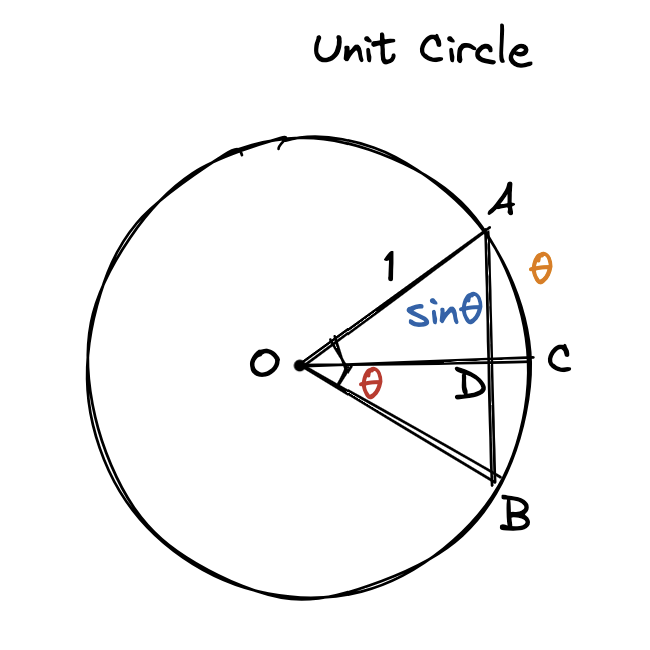
\includegraphics[scale=0.5]{images/circle_sinx.png}
    \caption{\(\sin x/ x\)的几何直观}\label{fig:sinx/x}
\end{figure}

弄清了  \(\sin x\) 在 \(x = 0\) 处的导数值,接着来处理 \(\cos x\) 在 \(x = 0\) 处的导数值。同样,从图 \ref{fig:(1-cosx)/x} 中可以得到以下结论:
\begin{align*}
    OB                   & = OA\cdot \cos \theta = r\cdot \cos \theta = \cos \theta \\
    BC                   & = OC - OB = r - OB = 1 - \cos \theta                     \\
    \overset{\frown}{AC} & = r \cdot \angle AOC = r \cdot \theta = \theta
\end{align*}

那么,同样 \(\cos x\) 在 \(x = 0\) 处的导数值就可以被表示为:
\begin{equation*}
    \left.\frac{d}{d\theta}\cos \theta\right|_{x=0} = \frac{BC}{\overset{\frown}{AC}} = \frac{1 - \cos \theta}{\theta}
\end{equation*}
同样,通过观察图 \ref{fig:(1-cosx)/x} 可以直观的看到,当 \(\theta \to 0\) 时,直线 \(BC\)和弧 \(\overset{\frown}{AC}\) 的长度均在减小,但是直线 \(BC\) 比弧 \(\overset{\frown}{AC}\) 减小的速度更快。即:当弧
\(\overset{\frown}{AC}\) 由 \(\theta \to \theta^{\prime}\)时(图中紫色部分),直线 \(BC\) 已经变得非常非常的短了(图中绿色部分)。所以可以得出:
\begin{equation}\label{eq:DerivativeofCosineatx=0}
    \frac{d}{d\theta}\cos \theta = \frac{BC}{\overset{\frown}{AC}} = 0 \quad \text{as} \quad \theta \to 0
\end{equation}
\begin{figure}[H]
    \centering
    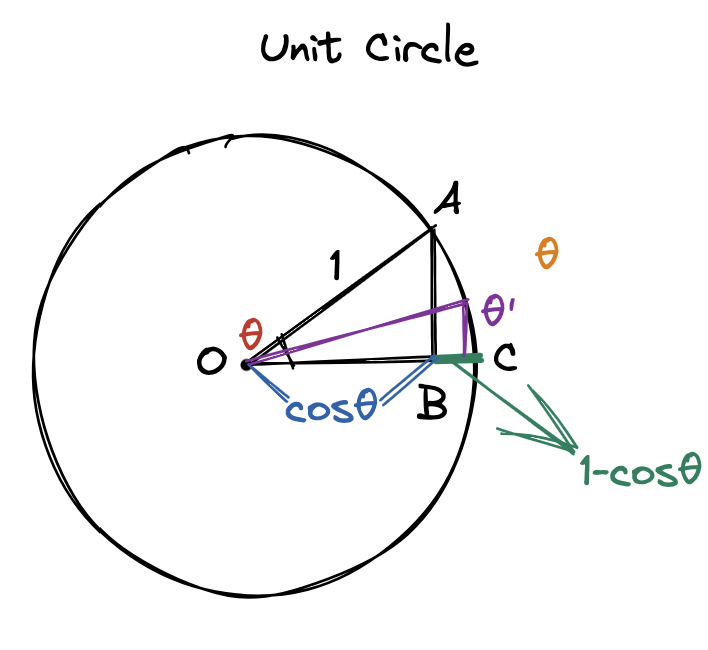
\includegraphics[scale=0.5]{images/circle_cosx.png}
    \caption{\((1-\cos x)/x\)的几何直观}\label{fig:(1-cosx)/x}
\end{figure}
到这,\(\sin x\) 和 \(\cos x\) 在 \(x = 0\) 处的导数值均被求出,可以回过头去求任意一点处 \(\sin x\) 的导数值。将 \(\sin x\) 在 \(x = 0\) 处的导数值(\ref{eq:DerivativeofSineatx=0}) 式 和 \(\cos x\) 在 \(x = 0\) 处的导数值 (\ref{eq:DerivativeofCosineatx=0}) 式,代入 (\ref{eq:DerivativeofSine}) 式,可以得到:
\begin{equation}\label{eq:DerivativeofSine_final}
    \frac{d}{dx}\sin x = 0 \cdot \sin x + 1 \cdot \cos x = \cos x
\end{equation}
同样,\(\cos x\) 在任意一点处的导数值,也可以通过同样的方式求出,下面就直接给出:
\begin{equation}\label{eq:DerivativeofCosine}
    \begin{aligned}
        \frac{d}{dx}\cos x
         & = \lim\limits_{\Delta x \to 0}\frac{\cos(x + \Delta x) - \cos x}{\Delta x}                                                                          \\
         & = \lim\limits_{\Delta x \to 0}\frac{\cos x \cos\Delta x - \sin x\sin\Delta x  - \cos x}{\Delta x}                                                   \\
         & = \lim\limits_{\Delta x \to 0}\left(\cos x\frac{\cos \Delta x - 1}{\Delta x}- \sin x \frac{\sin \Delta x}{\Delta x}\right)                          \\
         & = \cos x\lim\limits_{\Delta x \to 0}\frac{\cos \Delta x - 1}{\Delta x} - \sin x\lim\limits_{\Delta x \to 0}\frac{\sin \Delta x}{\Delta x} = -\sin x
    \end{aligned}
\end{equation}

除了上面这种,通过导数定义的方式去求 \(\sin x\) 和 \(\cos x\) 的导数,还可以通过几何的角度去求。下面以正弦函数\(\sin x\) 为例进行说明。

三角函数(或是周期函数)都可以用单位圆「unit circle」上的变化来表示,正如图 \ref{fig:derivativeofsine_geometric} 所展示的那样,正弦函数 \(\sin \theta\) 就可以被表示为线段 \(AC\),当 \(A\) 点绕圆周做循环往复的运动时,线段 \(AC\) 也随之发生相应的改变,正好对应着正弦函数 \(\sin \theta\) 的周期变化。

在 \ref{sec:Derivative's physics interpretation} 小节中曾提到过,导数的实质是要描述某个量的微小变化,正如图 \ref{fig:derivativeofsine_geometric} 所示,假设 \(A\) 点沿圆周运动到了 \(A^{\prime}\) 点(即:运动了 \(\Delta \theta\)),那么 \(AC\) (即:\(\sin \theta\)) 也发生了相应的改变,变化了 \(\Delta y\)。当 \(\Delta \theta\) 足够的小时,可以将其看成是微小变化,也就是导数,即:
\begin{equation*}
    \frac{d}{d\theta}\sin \theta = \frac{\Delta y}{\Delta \theta} \quad \text{as} \quad \Delta \theta \to 0
\end{equation*}
也就是说,需要求的其实是 \(\Delta y/\Delta \theta\) 的比值,观察图 \ref{fig:derivativeofsine_geometric} 可以发现,当 \(\Delta \theta\) 足够的小时,\(\Delta \theta\) 对应的弦 \(A^{\prime}A\)、弧 \(\overset{\frown}{A^{\prime}A}\)和过 \(A\) 点单位圆的切线(绿色虚线),三者趋近于重合,即可得出下面的结论:
\begin{equation*}
    \begin{aligned}
         & \frac{\Delta y}{\Delta \theta}  = \cos\angle A^{\prime}AD \\
         & \angle A^{\prime}AO             = \frac{\pi}{2}
    \end{aligned}
\end{equation*}
那么,现在需要做的就是从图 \ref{fig:derivativeofsine_geometric} 中,将 \(\angle A^{\prime}AD\) 给找出来。根据三角形一些简单的边角关系可以得到:
\begin{equation*}
    \begin{aligned}
         & \because \angle DA^{\prime}A + \angle A^{\prime}AD  = \frac{\pi}{2},\angle A^{\prime}AE+\angle EAO             = \frac{\pi}{2} \\
         & \because \angle DA^{\prime}A                        = \angle A^{\prime}AE                                                      \\
         & \therefore \angle A^{\prime}AD = \angle EAO                                                                                    \\
         & \because \angle EAO                                = \theta                                                                    \\
         & \therefore \angle A^{\prime}AD = \theta
    \end{aligned}
\end{equation*}
找出了  \(\angle A^{\prime}AD\),就可以得到正弦函数 \(\sin \theta\) 的导数值:
\begin{equation}
    \frac{d}{d\theta}\sin \theta = \frac{\Delta y}{\Delta \theta} = \cos\angle A^{\prime}AD = \cos \theta \quad \text{as} \quad \Delta \theta \to 0
\end{equation}
余弦函数 \(\cos \theta\) 的导数同样可以通过这样的几何的方式求出,由于方法和正弦函数 \(\sin \theta\) 类似就不重复赘述了。

\begin{figure}[H]
    \centering
    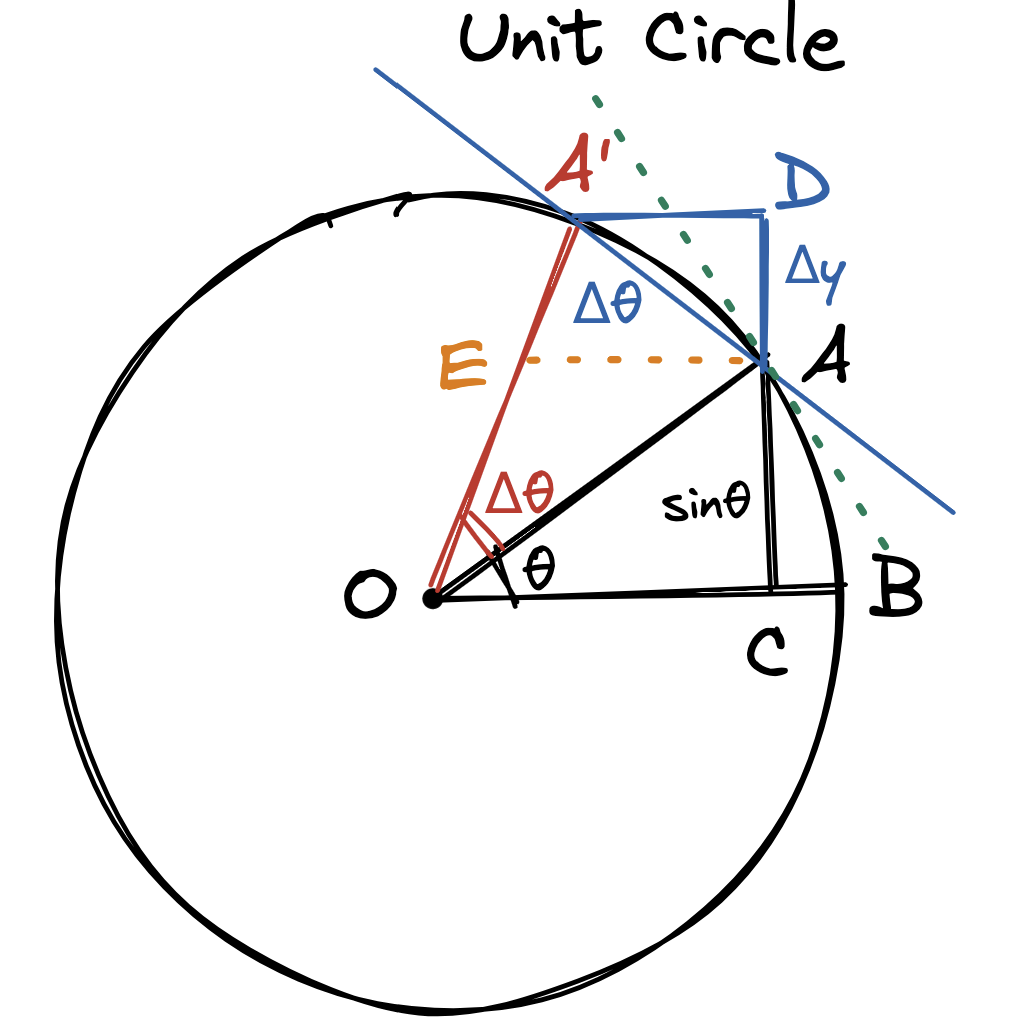
\includegraphics[scale=0.4]{images/derivativeofsine_geometric.png}
    \caption{\(\sin x\)导数的几何证明}
    \label{fig:derivativeofsine_geometric}
\end{figure}

得到了正弦函数 \(\sin(x)\) (\ref{eq:DerivativeofSine_final} 式) 和余弦函数 \(\cos(x)\) (\ref{eq:DerivativeofCosine} 式) 的导数,就可以求出正切函数 \(\tan(x)\) 的导数\footnote{余切函数 \(\cot(x)\) 的导数:\(\frac{d}{dx}cot(x) =\frac{d}{dx}\frac{1}{\tan(x)} = \frac{d}{dx}\frac{\cos(x)}{\sin(x)} = -\csc^{2}(x)\)}:
\begin{equation}\label{eq:DerivativeofTangent}
    \frac{d}{dx}\tan(x) =  \frac{d}{dx}\frac{\sin(x)}{\cos(x)} = \frac{\cos^{2}(x) + \sin^{2}(x)}{\cos^{2}(x)} = \sec^{2}(x)
\end{equation}
正割函数 \(\sec(x)\) 的导数:
\begin{equation}\label{eq:DerivativeofSecant}
    \frac{d}{dx}\sec(x) = \frac{d}{dx}\frac{1}{\cos(x)} = - \frac{1}{\cos^{2}(x)}(-\sin(x)) = \tan(x)\sec(x)
\end{equation}
以及余割函数 \(\csc(x)\) 的导数:
\begin{equation}\label{eq:DerivativeofCosecant}
    \frac{d}{dx}\csc(x) = \frac{d}{dx}\frac{1}{\sin(x)} = - \frac{1}{\sin^{2}(x)}(\cos(x)) = - \cot(x)\csc(x)
\end{equation}

\subsubsection{反三角函数}

在 \ref{sec:Implicit Differentiation} 小结中,提到了隐函数微分,它的最重要的一个应用就是求反函数\footnote{\(y = f(x) \Rightarrow x = g(y) \Rightarrow g(f(x)) = x, g = f^{-1}, f = g^{-1}\)}「Inverse Function」的导数。只要知道原函数导数,用隐函数微分就可以求出反函数导数。比如:在这一小节中要求的反三角函数的导数,就可以利用隐函数微分进行求导,因为在上一小节 \ref{sec:trigfunc} 中,已经得到了三角函数的导数。

\begin{myEx}
    \(y = \tan^{-1}x = \arctan x\)

    由于已知原函数导数,借助于原函数 \(\tan y  = x\),利用隐函数微分,求反函数 \(y = \tan^{-1}x\) 的导数。
    \begin{align*}
        % \frac{d}{dy}\left(\tan y  = x\right)
        \frac{d}{dx}\left(\tan y  = x\right)              \\
        \frac{d\left(\tan y\right)}{dy} \frac{dy}{dx} = 1 \\
    \end{align*}
    利用正切函数的导数公式(\ref{eq:DerivativeofTangent} 式)可以得到:
    \begin{align*}
        \sec^{2}y \frac{dy}{dx} = 1 \\
        \frac{dy}{dx} = \cos^{2}y
    \end{align*}
    根据如图 \ref{fig:Derivativeofarctanx} 所示三角形关系,可以得到:
    \begin{equation*}
        \cos y = \frac{1}{\sqrt{1 + x^{2}}}
    \end{equation*}
    所以最后可以得到,
    \begin{equation}
        \frac{d}{dx}\arctan x = \frac{1}{1 + x^{2}}
    \end{equation}
    \begin{figure}[H]
        \centering
        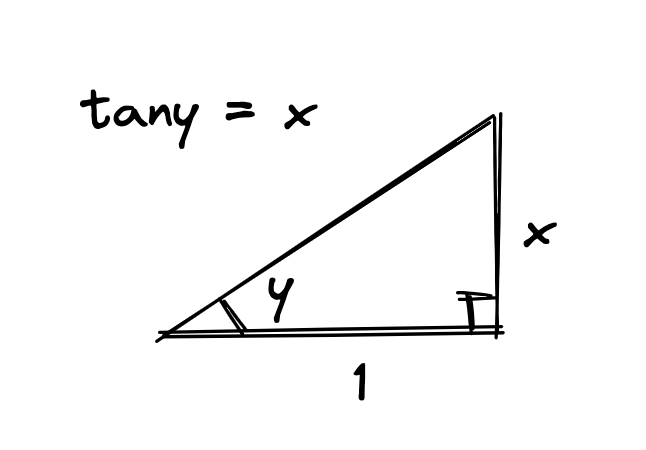
\includegraphics[scale=0.5]{images/Derivativeofarctanx.png}
        \caption{\(\tan(y) = x\)的三角形关系}
        \label{fig:Derivativeofarctanx}
    \end{figure}
\end{myEx}

\begin{myEx}
    \(y = \sin^{-1}(x) = \arcsin(x)\)

    同样,借助于 \(y = \sin^{-1}(x)\) 的反函数 \(\sin y = x\),利用隐函数微分,对其进行求导:
    \begin{align*}
        \frac{d}{dx}\left(\sin y = x\right) \\
        \cos y \frac{d}{dx}y = 1            \\
        \frac{d}{dx}y = \frac{1}{\cos y}
    \end{align*}
    利用到如图 \ref{fig:Derivativeofarcsinx} 所示的三角形关系,可以得到:
    \begin{equation*}
        \cos y = \sqrt{1 - x^2}
    \end{equation*}
    所以,最终可以得到:
    \begin{equation}
        \frac{d}{dx}\arcsin(x) = \frac{1}{\sqrt{1 - x^2}}\ (\left|x\right| < 1)
    \end{equation}
    \begin{figure}[H]
        \centering
        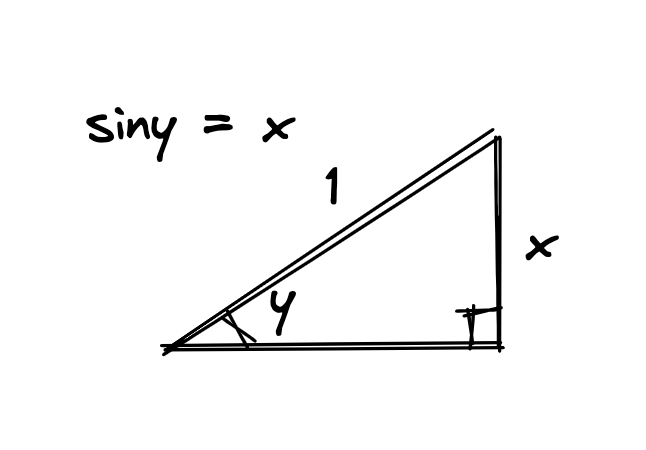
\includegraphics[scale=0.5]{images/Derivativeofarcsinx.png}
        \caption{\(\sin(y) = x\)的三角形关系}
        \label{fig:Derivativeofarcsinx}
    \end{figure}
\end{myEx}
同理,可以得到反余弦函数 \(y = \cos^{-1}(x) = \arccos(x)\) 的导数,下面不再赘述,直接给出结果:
\begin{equation}
    \frac{d}{dx}\arccos(x) = -\frac{1}{\sqrt{1-x^{2}}}\ (\left|x\right| < 1)
\end{equation}
注意,由于反三角函数和三角函数互为反函数,所以反三角函数的「定义域」就是对应三角函数的「值域」,反三角函数的「值域」就是对应三角函数的「定义域」\footnote{这条性质在所有互为反函数的函数对之间均成立.}。

\subsubsection{指数函数}\label{sec:ExponentialsFunc}

对于指数「exponentials」函数 \(a^{x}\) 的导数,根据导数的定义(Definition \ref{Def:Derivative}) 可以得到:
\begin{equation}\label{eq:DerivativeofExp}
    \frac{d}{dx}a^{x} = \lim\limits_{\Delta x \to 0}\frac{a^{x + \Delta x} - a^{x}}{\Delta x} = \lim\limits_{\Delta x \to 0}\frac{a^{x}\left(a^{\Delta x} - 1\right)}{\Delta x} = a^{x} \lim\limits_{\Delta x \to 0}\frac{a^{\Delta x} - 1}{\Delta x}
\end{equation}
从上面的式子中可以发现,指数函数 \(a^{x}\) 的导数与自身有关,它是自身的某一倍数,而这个倍数相对比较神秘与一个极限有关,不妨记作\(M(a)\),即:
\begin{equation}
    M(a) = \lim\limits_{\Delta x \to 0}\frac{a^{\Delta x} - 1}{\Delta x}
\end{equation}
那么指数函数 \(a^{x}\) 的导数定义式(\ref{eq:DerivativeofExp})就可以重写为:
\begin{equation}\label{eq:M(a)a^{x}}
    \frac{d}{dx}a^{x} = M(a)a^{x}
\end{equation}
现在,只要找到了 \(M(a)\),就能求出指数函数 \(a^{x}\) 在任意点的导数。

那么,\(M(a)\) 到底是什么?

下面,不妨学着 \ref{sec:trigfunc} 小节求三角函数的导数那样,先考虑在 \(x=0\) 处的指数函数的导数值,将 \(x=0\) 代入 (\ref{eq:M(a)a^{x}}) 式:
\begin{equation}\label{eq:DerivativeofExpAt0}
    \left.\frac{d}{dx}a^{x}\right|_{x=0} = M(a)
\end{equation}
根据上式的结果可以发现,\(M(a)\) 其实是指数函数 \(a^{x}\) 在 \(x=0\) 处的导数值。只要能够知道指数函数在一个地方的斜率(即:在 \(x=0\) 处的斜率),就能够由此导出函数在任意处的斜率。

但是,要知道知道指数函数在一个地方的斜率,就要能够对指数函数进行求导,而求导总绕不开 \(M(a)\) 的值,那么,有没有一个数\(a=a_{0}\) 能够使得 \(M(a_{0}) = 1\) \footnote{这里其实也可以定义一个数\(a_0\),使得\(M(a_{0}) = c,\quad c\text{为常数}\),\textcolor{green}{那为什么偏偏是\(1\)呢}?}呢?

下面,不妨定义某个像谜一样的底数 \(e\),使得:
\begin{equation} \label{eq:M(e)=1}
    M(e) = 1
\end{equation}
进一步将 (\ref{eq:M(e)=1}) 式分别代入 (\ref{eq:M(a)a^{x}}) 式以及 (\ref{eq:DerivativeofExpAt0}) 式,可以得到,底数 \(e\) 还满足:
\begin{equation}
    \begin{aligned}
        \frac{d}{dx}e^{x}                    & = e^{x}    \\
        \left.\frac{d}{dx}e^{x}\right|_{x=0} & = M(e) = 1
    \end{aligned}
\end{equation}
根据指数函数的性质\footnote{\(a^{x_1+x_2} = a^{x_1}a^{x_2}\),\ \ \((a^{x_1})^{x_2} = a^{x_1\cdot x_2}\),\ \ \(a = b^{log_{b}^{a}}\)},对于任意一个指数函数 \(a^{x}\),总可以将它表示成下面这样的形式:
\begin{equation}\label{eq:a^{x}=e^{xlna}}
    a^{x} = \left(e^{\ln a}\right)^{x} = e^{x\ln a}
\end{equation}
借助于指数函数 \(e^{x}\) 的导数,利用指数函数的性质(\ref{eq:a^{x}=e^{xlna}})式,可以对任意指数函数 \(a^{x}\) 进行求导:
\begin{equation}
    \frac{d}{dx}a^{x} = \frac{d}{dx} e^{x\ln a} = e^{x\ln a}\cdot \ln a = a^{x}\ln a
\end{equation}

在本节一开始的时候提到过,指数函数 \(a^{x}\) 的导数与自身成比例,即:指数函数 \(a^{x}\) 在 \(x=x_0\) 处的变化与 \(a^{x_0}\) 有关,这在实际生活中有很多的应用,很多与增长相关的现象都满足这一规律,比如:人口增长(某一年的人口增长总是与这一年人口的基数相关),经济增长(某一年的经济增长也总是和这一年的经济基础相关)等等,所以在建模时都会从指数模型出发。

在很多情况下,我们更关心的是在自身的基础上变化的比例,这时候可以借助于自然对数「Natural Log」,去简化计算:
\begin{align*}
    \frac{d}{dx}a^{x}                  & = a^{x}\cdot \ln a          \\
    \frac{d}{dx}\ln \left(a^{x}\right) & =\ln a\frac{d}{dx}x = \ln a
\end{align*}
当然,这个技巧不光针对指数函数,它适用于任何导数与自身成比例的函数,比如下面这个例子。
\begin{myEx}
    \(\frac{d}{dx}\sec x = \sec x \tan x\)

    显然,\(\sec x\) 的导数与自身成比例,那么当对 \(\sec x\) 取对数时,它的导数就会满足:
    \begin{equation*}
        \frac{d}{dx}\ln \sec x = \tan x
    \end{equation*}
\end{myEx}

\subsubsection{对数函数}

在 \ref{sec:ExponentialsFunc} 小节中,定义了一个独特的数字 \(e\),下面,引入自然对数\footnote{对数的定义:\(y=e^{x}\Leftrightarrow \ln y =x\),与指数互为逆运算.}「Natural Log」\footnote{所谓自然对数,无需任何参考就会自然产生,具有自然属性.}:
\begin{equation}
    w = \ln (x)
\end{equation}
由于在 \ref{sec:ExponentialsFunc} 小节中给出了指数函数的导数,而对数与指数之间互为逆运算,所以借助于隐函数微分,可以对自然对数函数进行求导:
\begin{align*}
    w & = \ln (x)  \Rightarrow e^{w}  = x   \\
      & \frac{d}{dx}\left(e^{w}  = x\right) \\
      & e^{w}\frac{d}{dx}w = 1              \\
      & \frac{d}{dx}w = \frac{1}{e^{w}}
\end{align*}
最终,可以得到自然对数 \(w = \ln (x)\) 的导数为:
\begin{equation}
    \frac{d}{dx}\ln (x) = \frac{1}{x}
\end{equation}

得到了自然对数 \(w = \ln (x)\) 的导数,可以引入一种新的求导技巧——对数微分法,适用于求导的表达式中出现很多项连乘以及在某些项中出现指数的情况。

\begin{myEx}
    用对数微分法重新求解指数函数 \(a^{x}\) 的导数:\(\frac{d}{dx}a^{x}\)

    令 \(u = a^{x}\),那么:
    \begin{align*}
        \ln u = x \ln a                          \\
        \frac{d}{dx}\left(\ln u = x \ln a\right) \\
        \frac{1}{u}\frac{d}{dx}u = \ln a         \\
        \frac{d}{dx}u  = u \ln a                 \\
    \end{align*}
    最后,再把 \(u = a^{x}\) 代入,可以得到:
    \begin{equation*}
        \frac{d}{dx}a^{x}  = a^{x} \ln a
    \end{equation*}
\end{myEx}

\begin{myEx}
    \(V = x^{x}\)

    对 \(V = x^{x}\) 左右两边取对数,有:
    \begin{align*}
        \ln V = x \ln x
    \end{align*}
    再对 \(\ln V = x \ln x\) 等式两边同时求导:
    \begin{align*}
        \frac{1}{V}\frac{d}{dx}V & = \ln x + 1               \\
        \frac{d}{dx}V            & = V\left(\ln x + 1\right)
    \end{align*}
    最后,将 \(V = x^{x}\) 再代入等式,有:
    \begin{equation}
        \frac{d}{dx}x^{x} = x^{x}\left(\ln x + 1\right)
    \end{equation}
\end{myEx}

\begin{myEx}
    \(\lim\limits_{n\to \infty}\left(1 + \frac{1}{n}\right)^{n}\)

    令 \(u = \left(1 + \frac{1}{n}\right)^{n}\),对 \(u\) 取对数,有:
    \begin{equation*}
        \ln u = n \ln \left(1 + \frac{1}{n}\right)
    \end{equation*}
    令 \(\Delta x = \frac{1}{n}\),其中,\(n\to \infty\),\(\Delta x \to 0\),有:
    \begin{equation*}
        \ln u = \frac{\ln \left(1 + \Delta x\right)}{\Delta x} = \frac{\ln \left(1 + \Delta x\right) + \ln(1)}{\Delta x} = \left.\frac{d}{dx}\ln x\right|_{x = 1} = \left.\frac{1}{x}\right|_{x = 1} = 1
    \end{equation*}
    最后,对 \(\lim\limits_{n\to \infty}\left(1 + \frac{1}{n}\right)^{n}\) 进行等价变化,有:
    \begin{equation}
        \lim\limits_{n\to \infty}\left(1 + \frac{1}{n}\right)^{n} = \lim\limits_{n\to \infty}\left[e^{\ln \left(1 + \frac{1}{n}\right)}\right]^{n} = \lim\limits_{n\to \infty}e^{n\ln \left(1 + \frac{1}{n}\right)} = e^{\lim\limits_{n\to \infty} n\ln \left(1 + \frac{1}{n}\right)} = e
    \end{equation}
\end{myEx}
从这个例子中,可以发现 \(e\) 是真实存在的,并且找的了逼近 \(e\) 的方法:
\begin{equation}
    e = \lim\limits_{n\to \infty}\left(1 + \frac{1}{n}\right)^{n}
\end{equation}
注意:“\(=\)” 所表示的关系永远是双向的,就拿上面这个等式来说,从左往右看,表示 \(e\) 可以用 \(\lim\limits_{n\to \infty}\left(1 + \frac{1}{n}\right)^{n}\) 来近似,而从右往左看,表示 \(\lim\limits_{n\to \infty}\left(1 + \frac{1}{n}\right)^{n}\) 的极限为 \(e\),不同的角度关注的重点不同。

\subsubsection{幂函数}

幂函数的导数「the derivative of the powers」:
\begin{equation}
    \frac{d}{dx}x^{r} = rx^{r-1}, \ \text{其中,} r\in R
\end{equation}
\begin{proof}
    \(\frac{d}{dx}x^{r} = rx^{r-1}\)

    方法一(base e):
    \begin{align*}
        x^{r}                                      & = \left(e^{\ln x}\right)^{r} = e^{r\ln x}                           \\
        \frac{d}{dx}x^{r} = \frac{d}{dx}e^{r\ln x} & = e^{r\ln x} \cdot \frac{r}{x} = x^{r} \cdot \frac{r}{x} = rx^{r-1}
    \end{align*}

    方法二(log diff):

    令 \(u = x^{r}\),并对 \(u\) 取对数,有:
    \begin{equation*}
        \ln u = r\ln x
    \end{equation*}
    对等式左、右两边同时求导,可得:
    \begin{align*}
        \frac{1}{u}\frac{d}{dx}u & = \frac{r}{x}  \\
        \frac{d}{dx}u            & = u\frac{r}{x}
    \end{align*}
    最后,将 \(u = x^{r}\) 代入,可以得到:
    \begin{equation*}
        \frac{d}{dx}x^{r} = x^{r}\frac{r}{x} = rx^{r-1}
    \end{equation*}
\end{proof}

其实,在前面已经涉及到了部分幂函数的导数(当 \(r \in Z\)时,Example \ref{Ex:x^{n}} 和 \ref{Ex:1/x} 以及 当 \(r \in Q\)时,Example \ref{Ex:x^{m/n}}),但是还缺少当 \(r\) 为无理数的情况,现在算是集齐了幂函数的导数的最后一块拼图。

%% 参考文献
\newpage
\nocite{CalculusSingleVariable}
\bibliography{references}

\end{document}